
\documentclass[11pt]{article}
\usepackage[margin=0.78in]{geometry}
\usepackage{booktabs}
\usepackage{array}
\usepackage{graphicx}
\usepackage{float}
\usepackage{hyperref}
\hypersetup{colorlinks=true, linkcolor=blue, urlcolor=blue}
\setlength{\parskip}{0.45em}
\setlength{\parindent}{0pt}
\renewcommand{\arraystretch}{1.12}

\title{Rolling ML Quality-Gate Comparison\\\large Base vs Filtered TP2 Universes}
\author{ML-Based Trading of TP2-Inspired Violations in SPY American Call Options}
\date{June 22, 2026}

\begin{document}
\maketitle

\section{Purpose}

This report compares the current rolling LightGBM five-action model across
three point-in-time candidate universes: the base conservative bid/ask TP2
universe, the volume-and-delta universe, and the strict market-quality universe.
All runs use the same 3-year train, 1-year validation, 1-year test folds and the
same net-P\&L target.

\section{Aggregate Results}
\begin{tabular}{lrrrrrrrr}
\toprule
Gate & Rows after gate & Selected & Executed & Invalid & Exec rate & Hit rate & Net P\&L & Positive years \\
\midrule
Base & 226,577 & 14,874 & 8,672 & 6,202 & 58.3\% & 50.3\% & \$1.99M & 4 \\
Volume + Delta & 15,772 & 1,865 & 1,720 & 145 & 92.2\% & 55.2\% & \$5.7K & 4 \\
Strict Quality & 8,953 & 1,650 & 1,489 & 161 & 90.2\% & 61.3\% & \$195.0K & 4 \\
\bottomrule
\end{tabular}
\begin{figure}[H]
  \centering
  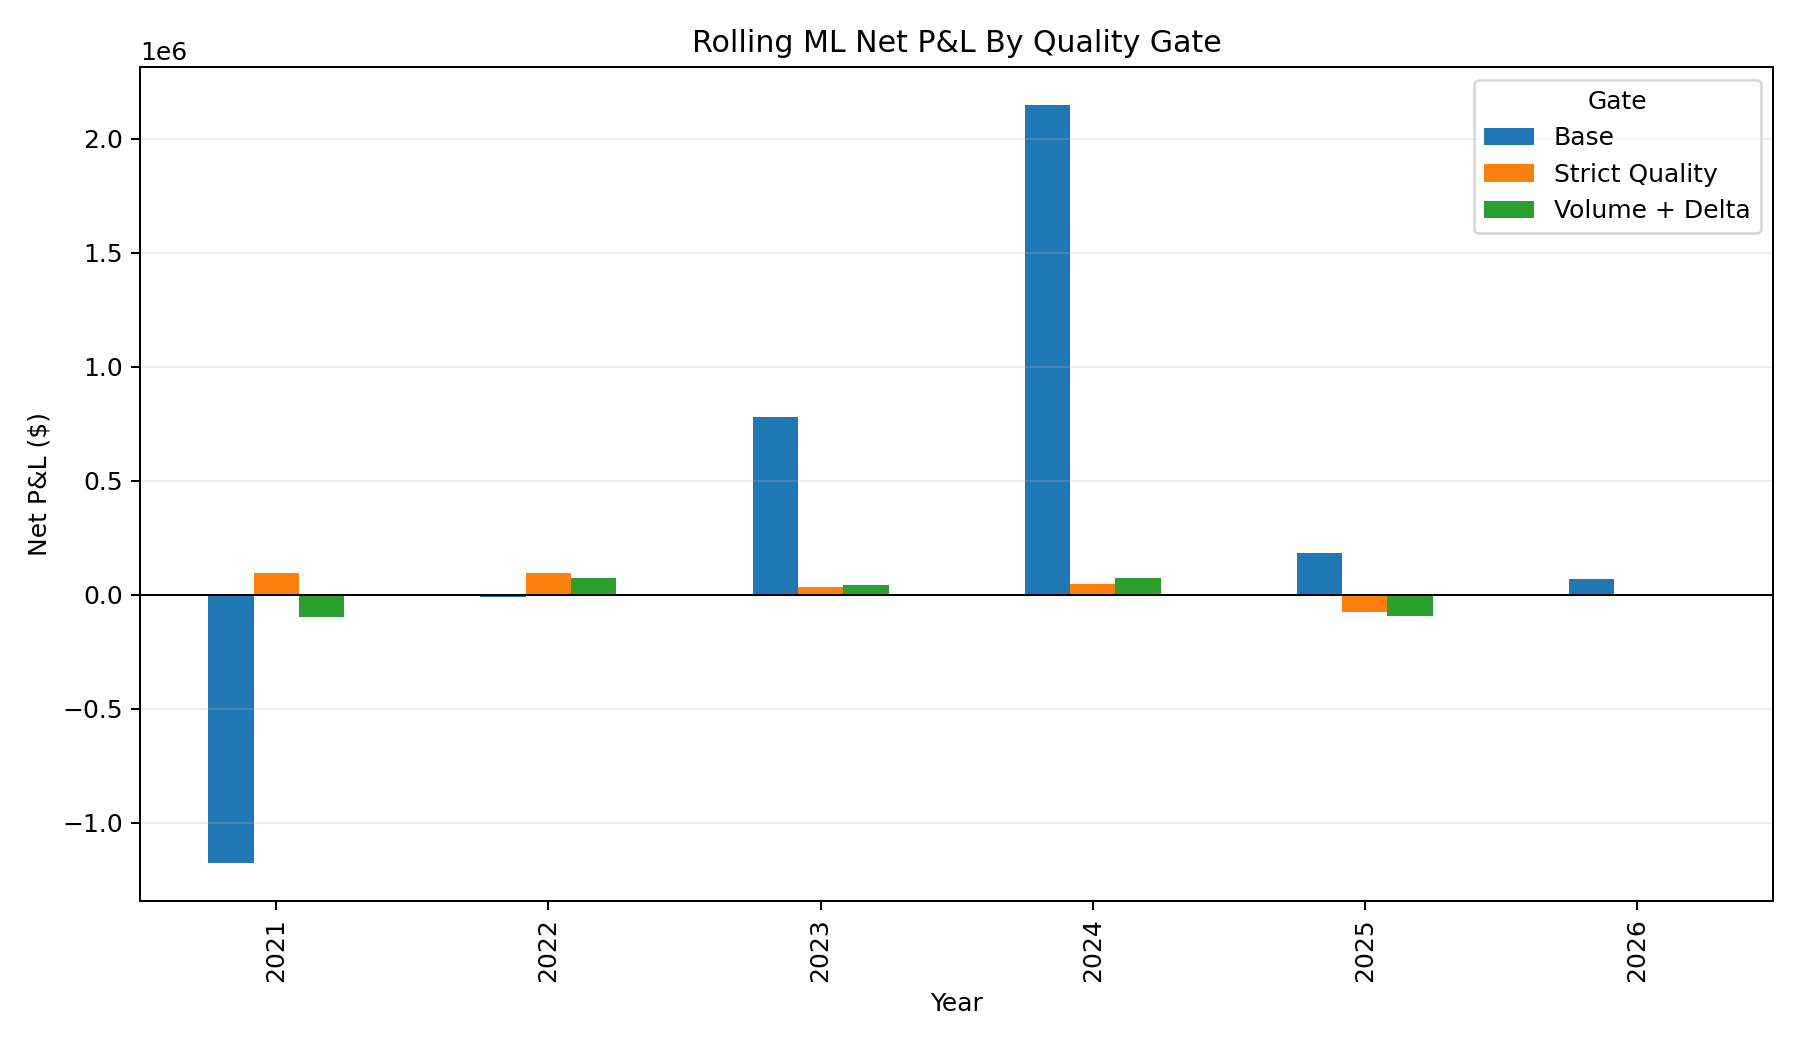
\includegraphics[width=0.92\linewidth]{figures/ml_quality_gate_yearly_pnl.png}
  \caption{Test-year rolling net P\&L by quality gate.}
\end{figure}

\begin{figure}[H]
  \centering
  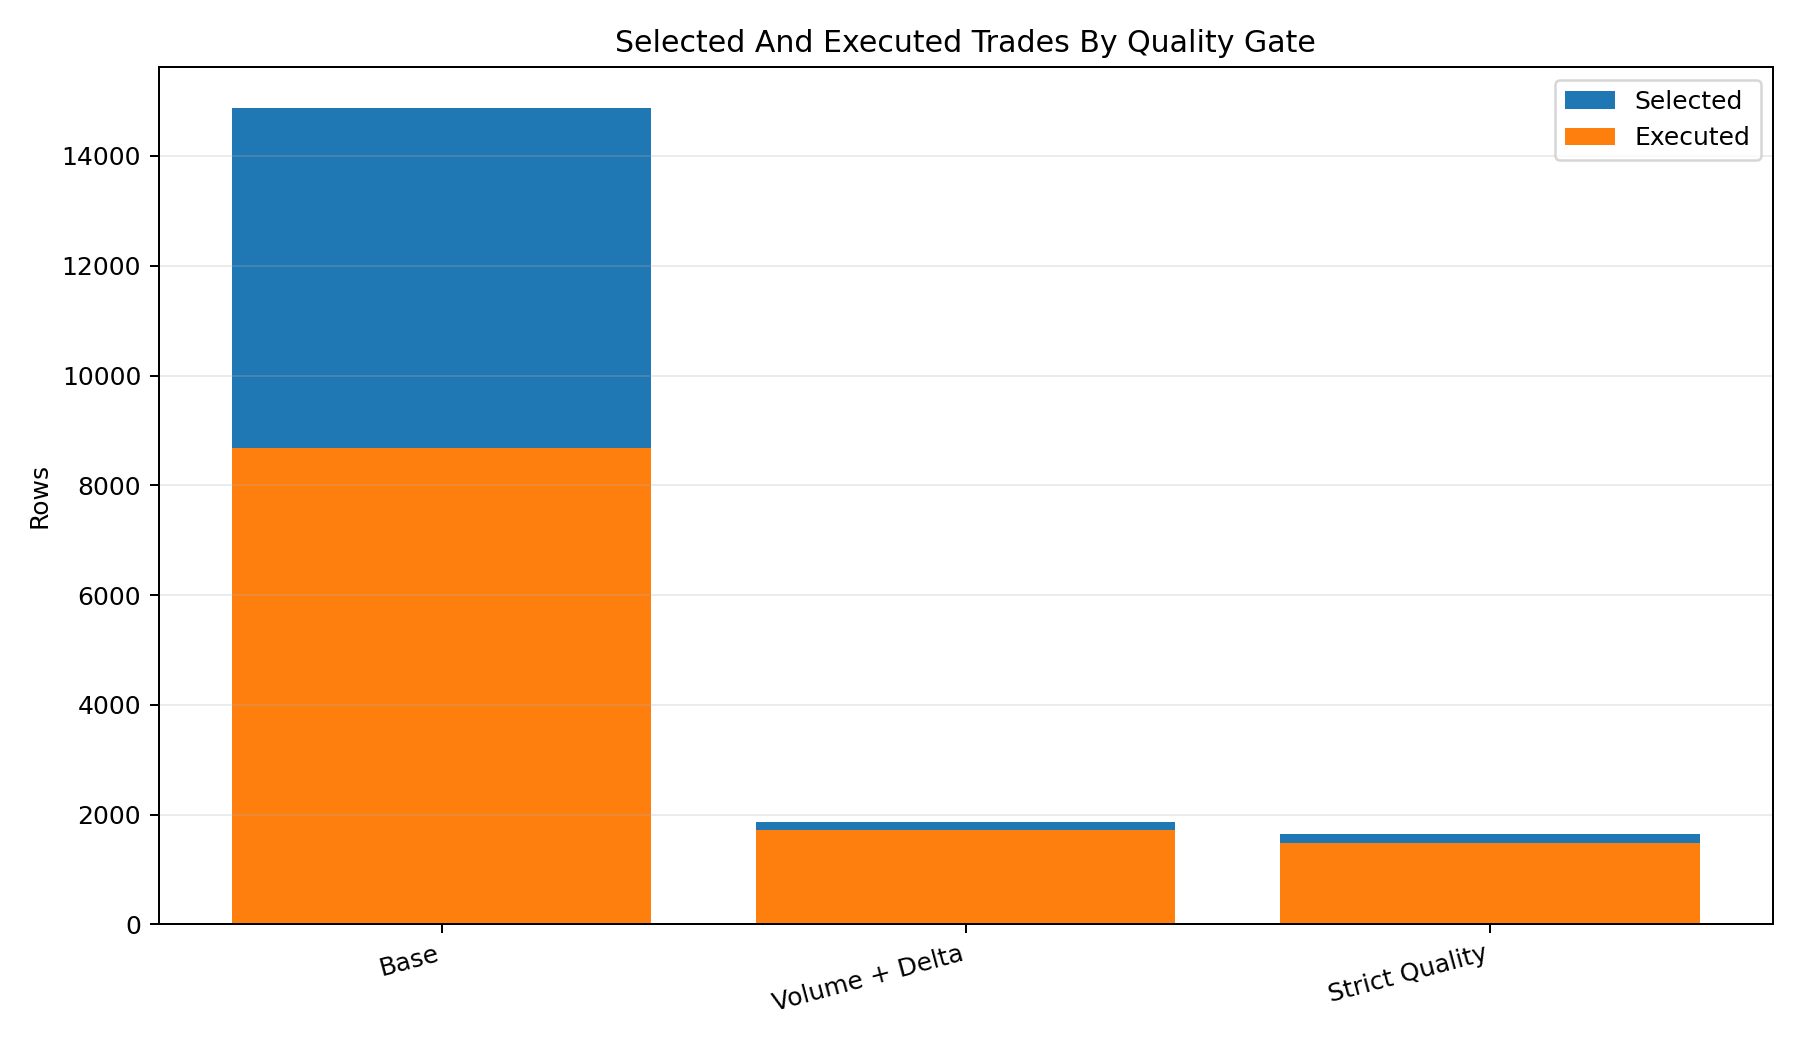
\includegraphics[width=0.92\linewidth]{figures/ml_quality_gate_trade_counts.png}
  \caption{Selected and executed trade counts by quality gate.}
\end{figure}


\section{Yearly Detail}
\begin{tabular}{lrrrrrrrr}
\toprule
Gate & Year & Rows & Selected & Executed & Invalid & Hit rate & Net P\&L & Threshold \\
\midrule
Base & 2021 & 20,588 & 392 & 384 & 8 & 23.2\% & -\$1.18M & 0.800 \\
Base & 2022 & 6,604 & 1,077 & 979 & 98 & 43.3\% & -\$10.1K & 0.475 \\
Base & 2023 & 12,731 & 763 & 435 & 328 & 62.3\% & \$778.2K & 0.050 \\
Base & 2024 & 34,167 & 5,134 & 2,912 & 2,222 & 61.7\% & \$2.15M & 0.325 \\
Base & 2025 & 41,577 & 3,542 & 2,373 & 1,169 & 62.0\% & \$183.9K & 0.050 \\
Base & 2026 & 9,335 & 3,966 & 1,589 & 2,377 & 19.7\% & \$70.7K & 0.275 \\
Volume + Delta & 2021 & 1,157 & 754 & 710 & 44 & 40.8\% & -\$96.1K & 0.050 \\
Volume + Delta & 2022 & 932 & 568 & 557 & 11 & 69.7\% & \$74.7K & 0.475 \\
Volume + Delta & 2023 & 571 & 242 & 235 & 7 & 66.0\% & \$44.0K & 0.050 \\
Volume + Delta & 2024 & 288 & 179 & 136 & 43 & 56.6\% & \$75.0K & 0.050 \\
Volume + Delta & 2025 & 412 & 121 & 81 & 40 & 46.9\% & -\$92.4K & 0.600 \\
Volume + Delta & 2026 & 70 & 1 & 1 & 0 & 100.0\% & \$414 & 0.700 \\
Strict Quality & 2021 & 792 & 515 & 477 & 38 & 47.8\% & \$96.8K & 0.050 \\
Strict Quality & 2022 & 735 & 659 & 641 & 18 & 72.2\% & \$93.6K & 0.300 \\
Strict Quality & 2023 & 145 & 145 & 144 & 1 & 66.7\% & \$32.8K & 0.050 \\
Strict Quality & 2024 & 177 & 128 & 100 & 28 & 62.0\% & \$48.0K & 0.275 \\
Strict Quality & 2025 & 293 & 203 & 127 & 76 & 50.4\% & -\$76.2K & 0.450 \\
Strict Quality & 2026 & 38 & 0 & 0 & 0 & NA & \$0 & 0.725 \\
\bottomrule
\end{tabular}

\section{Interpretation}

The base universe remains the primary sample because it has broad coverage and
positive aggregate out-of-sample P\&L, but it includes many low-quality episodes.
The volume-and-delta universe is cleaner but much smaller and produces mixed
rolling results. The strict-quality universe has the cleanest label universe but
is too sparse in recent years, especially 2026, so it should be treated as a
robustness diagnostic rather than a main model sample.

For the paper, this supports a layered empirical design: report the base model
as the main rolling result, then use volume/delta and strict-quality filtered
runs to show how sensitive the ML edge is to market-quality assumptions.

\end{document}
